\documentclass[french,english]{article}
\usepackage[T1]{fontenc}
\usepackage[utf8]{inputenc}
\usepackage{fixltx2e}
\usepackage{graphicx}
% \usepackage{listings}
\usepackage{babel}
\usepackage{color}
\usepackage{colortbl}

\definecolor{Gray}{gray}{0.85}

\begin{document}
  \section{Brouillon}
  \begin{figure}
    \begin{center}
      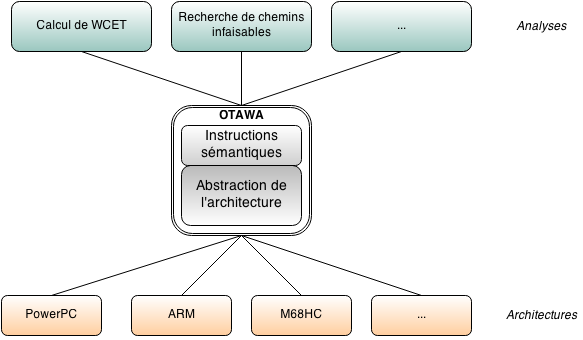
\includegraphics[scale=0.5]{pictures/otawa_abstraction_architecture.png}
    \end{center}
    \caption{OTAWA permet aux analyses de s'abstraire de l'architecture}
  \end{figure}
  \begin{figure}   
    \begin{tabular}{|l|l|} \hline
      \textbf{Instruction} & \textbf{Sémantique}\\ \hline \hline
      \texttt{NOP} & (rien)\\ \hline
      \texttt{BRANCH} & \\
      \texttt{TRAP} & Indicateurs du flot du programme\\
      \texttt{CONT} & \\ \hline
      \texttt{IF cond sr jump} & si la condition \texttt{cond} sur le registre \texttt{sr} est vraie, continuer,\\
      & sinon sauter \texttt{jump} instructions\\ \hline
      \texttt{LOAD reg addr type} & reg $\leftarrow$ \texttt{MEM\textsubscript{type}} \\ \hline
      \texttt{STORE reg addr type} & \texttt{MEM\textsubscript{type}} $\leftarrow$ \texttt{reg}\\ \hline
      \texttt{SCRATCH d} & \texttt{d $\leftarrow$ $\top$} \textit{(invalidation)}\\ \hline
      \texttt{SET d a} & \texttt{d $\leftarrow$ a}\\ \hline
      \texttt{SETI d cst} & \texttt{d $\leftarrow$ cst}\\ \hline
      \rowcolor{Gray} \texttt{SETP d cst} & \texttt{page(d) $\leftarrow$ cst}\\ \hline
      \texttt{CMP d a b} & \texttt{d $\leftarrow$ a $\sim$ b}\\ \hline
      \rowcolor{Gray} \texttt{CMPU d a b} & \texttt{d $\leftarrow$ a $\sim$\textsubscript{unsigned} b}\\ \hline
      \texttt{ADD d a b} & \texttt{d $\leftarrow$ a $+$ b}\\ \hline
      \texttt{SUB d a b} & \texttt{d $\leftarrow$ a $-$ b}\\ \hline
      \rowcolor{Gray} \texttt{SHL d a b} & \texttt{d $\leftarrow$ unsigned(a) <{<} b}\\ \hline
      \rowcolor{Gray} \texttt{SHR d a b} & \texttt{d $\leftarrow$ unsigned(a) >{>} b}\\ \hline
      \texttt{ASR d a b} & \texttt{d $\leftarrow$ a >{>} b}\\ \hline
      \texttt{NEG d a} & \texttt{d $\leftarrow$ $-$a}\\ \hline
      \rowcolor{Gray} \texttt{NOT d a} & \texttt{d $\leftarrow$ $\neg$a}\\ \hline
      \rowcolor{Gray} \texttt{AND d a b} & \texttt{d $\leftarrow$ a \& b}\\ \hline
      \rowcolor{Gray} \texttt{OR d a b} & \texttt{d $\leftarrow$ a | b}\\ \hline
      \rowcolor{Gray} \texttt{XOR d a b} & \texttt{d $\leftarrow$ a $\oplus$ b}\\ \hline
      \texttt{MUL d a b} & \texttt{d $\leftarrow$ a $\times$ b}\\ \hline
      \rowcolor{Gray} \texttt{MULU d a b} & \texttt{d $\leftarrow$ unsigned(a) $\times$ unsigned(b)}\\ \hline
      \texttt{DIV d a b} & \texttt{d $\leftarrow$ a / b}\\ \hline
      \rowcolor{Gray} \texttt{DIVU d a b} & \texttt{d $\leftarrow$ unsigned(a) / unsigned(b)}\\ \hline
      \texttt{MOD d a b} & \texttt{d $\leftarrow$ a \% b}\\ \hline
      \rowcolor{Gray} \texttt{MODU d a b} & \texttt{d $\leftarrow$ unsigned(a) \% unsigned(b)}\\ \hline
      \rowcolor{Gray} \texttt{SPEC} & (instruction spéciale non supportée par OTAWA)\\ \hline
    \end{tabular}
    \textit{En gris : les instructions qui ne sont pas (encore) traitées par notre analyse.}
    \caption{Liste des instructions sémantiques d'OTAWA} 
  \end{figure}


  \section{Objectif}
  \subsection{WCET, enjeux (systèmes critiques etc)}
  Améliorer l'estimation de WCET

  \section{Solution}
  Explication : calcul de WCET par IPET, max d'un système ILP\\
  Solution = Recherche de chemins infaisables pour améliorer l'estimation du WCET\\
  Parler des outils choisis (OTAWA + CVC4 ?)\\
  
  \section{Structures de données utilisées}
  La représentation des prédicats (associés à un Edge)\\
  => représentation également de la mémoire\\
  Traduction des prédicats dans le solveur SMT

  \section{Structure de l'algorithme}
  CFG : Représentation du programme sous la forme de graphe\\
  On parcourt tous les chemins\\
  On les représente sous la forme de prédicats (on y associe un arc du CFG\\
  On fait des appels au SMT pour vérifier la satisfiabilité\\
  Retourne la liste de prédicats\\
  On génère les contraintes ILP\\
\end{document}
